\section{Ziel}
In diesem Versuch soll die Verdampfungswärme L, ihre Temperaturabhängigkeit sowie die Dampfdruckkurve
von Wasser ebenso wie von einer anderen Substanz bestimmt werden.
\section{Theorie}
\label{sec:Theorie}
\cite{sample}
Einem Stoff kann in nahezu jeder Kombinationen aus Druck $p$ und Temperatur $T$ eine eindeutig definierte Phase zugeorndet werden.
Im Allgemeinen wird zwischen den Phasen fest, flüssig und gasförmig unterschieden. Zwischen diesen Zuständen verlaufen jeweils
sogenannte Dampfdruckkurven. An jedem Punkt, welcher auf der Kurve liegt, koexistieren die zwei Zustände, welche sich jeweils neben der Kurve befinden.
Visualisiert  wird das ganze in einem Zustandsdiagramm. Ebenso sind die Punkte "TP" \, sowie "KP" \, wichtig zu erläutern. Der Tripelpunkt(TP) beschreibt die Kombination
aus $p$ und $T$, an der alle drei Phasen koexistieren. Von hier aus startet die zwischen der gasförmigen und flüssigen Phase verlaufenden Dampfdruckkurve und
endet am kritischen Punkt(KP). Entlang dieser Kurve hat das System nur noch den Freheitsgrad  $T$, da zu jeder Temperatur ein Druck festgelegt ist.
\begin{figure}[h]
    \centering
    \includegraphics[scale=0.8]{"screen.jpg"}
    \caption{Qualitatives Zustandsdiagramm des Wassers. Der Druck $p$ ist gegen die Temperatur $T$ aufgetragen.}
    \label{Abb1:Zustandsdiagramm}
\end{figure}
\noindent
Eine weitere wichtig einzuführende Größe ist die molare Verdampfungswärme $L$. Durch diese wird die Menge an Energie beschrieben, die benötigt wird, den Phasenübergang
eines Teilchens von flüssig zu gasgförmig zu bewirken.
Daher ist sie maßgebend für den Verlauf der Dampfdruckkurve. In dem Messbereich
unter einem Bar wird L als Konstante angenommen.\\
Aus der Thermodynamik ist bekannt, dass die Temperatur eines Stoffes über die gemittelte Stoßzeit eines Teilchens definiert ist. Die Teilchen
mit der kürzesten mittleren Stoßzeit, sind auch jene mit der größten kinetischen Energie. Soll ein Stoff also zum dampfen gebracht werden, muss ihm Energie zugeführt werden.
Hat ein Teilchen genug kinetische Energie, erfährt es einen Phasenübergang - der Stoff verdampft. Für dieses Phänomen
wird genau die Energiemenge $L$ benötigt. Der Phasenübergang bewirkt ebenfalls einen Anstieg des Drucks im Gas oberhalb der Flüssigkeit.\\
Nach langer Zeit stellt sich ein Gleichgewicht zwischen verdampfenden und kondensierenden Teilchen ein. Der so erreichte Druck im Dampf
wird als Sättigungsdampfdruck definiert. Dieser ist nicht abhängig vom Volumen, welches von dem Dampf ausgefüllt wird. Ändert sich dieses Volumen, wird nicht der Druck, sondern das Gleichgewicht verändert. 
Daher gilt die ideale Gasgleichung
pV=RT nicht.\\
Im Folgenden soll eine Differentialgleichung bestimmt werden, welche zur Bestimmung der Dampfdruckkurve geeignet ist.
Dazu muss folgender Kreisprozess für ein Mol mathematisch näher betrachtet werden.
\begin{figure}[h!]
    \centering
    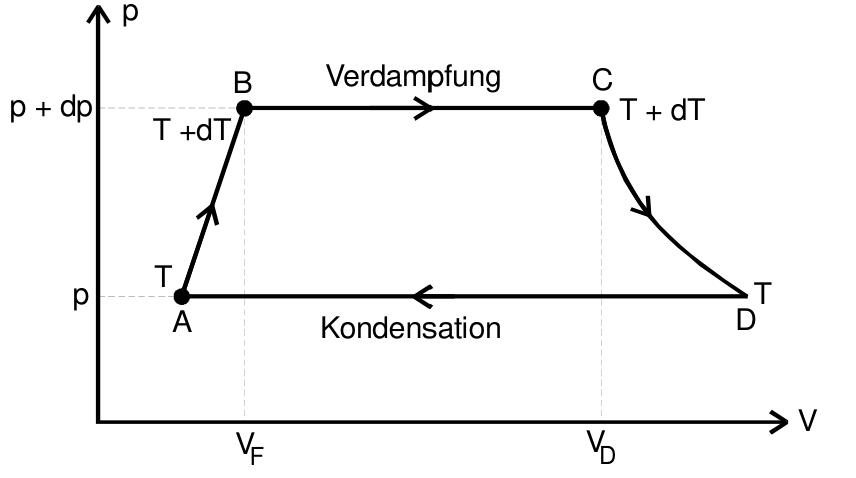
\includegraphics[scale=0.8]{sreen2.jpg}
    \caption{Kreisprozess für Verdampfung und Kondensation eines Stoffes. Der Druck p ist
    gegen das Volumen V dargestellt.}
    \label{Abb2:Kreisprozess}
\end{figure}
\\
Durch Überlegungen am Kreisprozess ergibt sich die Clausius-Clapeyronsche Gleichung 
\begin{equation}
    (V_D-V_F)dp=\frac{L}{T}dT.
\end{equation}
Es sind zwei Ausdrücke für die gesamt geleistete Arbeit miteinander gleichgesetzt, 
die sich auf der einen Seite aus der Volumendifferenz von Punkt B zu Punkt C sowie einer infitisimalen
Druckänderung ergibt.
Rechts beschreibt der Quotient der Verdampfungswärme mit der Temperatur um eine infinitesimal kleine
Temperaturänderung die Gesamtarbeit.\\
Unter der Bedingung, dass $V_D$, $V_F$ und $L$ konstant seien, ist diese Gleichung direkt lösbar. Dies ist im
Allgemeinen jedoch nur in wenigen Temperaturbereichen möglich. Hier wird der Fall behandelt, dass $T$ deutlich kleiner
als die kritische Temperatur $T_\text{Kr}$ ist.
\newpage
Somit sind folgende Annahmen zu treffen:
\begin{itemize}
    \item[1.] $V_F<<V_D$. Daher darf $V_F$ vernachlässigt werden.
    \item[2.] Für $V_D$ gilt die ideale Gasgleichung: $V_D(p,T)=\frac{T}{p}$
    \item[3.] L darf keine Abhängigkeit von Druck $p$ oder Temperatur $T$ haben. Damit
    ergibt sich als Lösung der DGL: $p=p_0\cdot \exp(-\frac{1}{T}\cdot\frac{L}{R})$
\end{itemize}
Es existiert also eine Proportionalität zwischen der Teilchenanzahl in der Dampfphase sowie
des Drucks oberhalb der Flüssigkeit. Wie bereits diskutiert, braucht ein Teilchen jedoch eine bestimmte
kinetische Energie zum Phasenübergang, was durch die Boltzmann-Statistik beschrieben wird.
Über die Gesamtenergie $W$ ergibt sich für den Anteil der Moleküle, die in die Dampfphase übergehen können:
\begin{equation*}
\exp(-W/kT)\Rightarrow p\propto \exp(-W/kT).
\end{equation*}